\documentclass[a4paper]{article}
\usepackage{graphicx}
\usepackage{onecolceurws}
\usepackage{csquotes}
\usepackage{hyperref}
\usepackage{framed}
\usepackage{mdframed}
\usepackage{upquote}
\usepackage{lmodern}
\usepackage[normalem]{ulem}

\title{Sophize Markdown and Collaboration Interface }

\author{
Abhishek Chugh
}

\institution{ Sophize Foundation\\
                Bengaluru, India \\ abc@sophize.org }


\begin{document}
\maketitle

\begin{abstract}
We have extended the Markdown language to represent the connections between mathematical objects that exist across various sources of knowledge. Using the new language, we demonstrated an interactive interface that helps its users explore mathematics content on the web. We also utilized this new language to create a novel communication system built specifically to aid mathematicians in solving problems collaboratively. This contribution sketches the basic ideas and provides links to some demos of the new functionality.

\end{abstract}

\vskip 32pt

 

\section{Introduction}


Sophize is a novel mathematics library and discussion platform. Our primary mission is to help users find existing proofs of mathematical statements, to discover new proofs, and to utilize this knowledge in their work. Mathematical proofs can be seen as directed acyclic graphs of logical arguments that can extend across a large number of documents and databases. These proofs are carried out based on a variety of foundations such as ZFC, intuitionistic logic and type theory. The arguments used in any proof are considered valid  or not based on criteria that can vary. Most academic mathematics is peer-reviewed and published, but some mathematical proofs can be found in community curated sources such as Wikipedia. Proofs can also be algorithmically generated, and at the highest level of verification, they are represented and verified using a formal system. Thus, aggregating proofs from such a wide variety of sources that use a wide variety of foundations and verification criteria is a challenging problem that requires novel knowledge organization techniques and user interfaces. This article focuses on these user interfaces that help users to navigate and understand existing proofs and discover new ones.  Our work can also be seen as a step towards formalizing the network of information that exists in the connections of mathematical objects. The committee on planning a global library of the mathematical sciences recognized that this network is largely unexplored, and formalizing it has tremendous potential to accelerate math research\cite{sciences2014developing}. This introductory video gives an overview of how structured knowledge can help: \url{https://youtu.be/Wb1JbW9Otek}.



In this paper, we first discuss the details of Sophize Markdown, an extension of the Markdown language. It is convenient enough to be used for a casual discussion of mathematical ideas over the web. It is also powerful enough to embed mathematical entities such as definitions, theorems, and proofs from a wide variety of sources, including formal languages. Then, we elaborate on the communication interface designed to help mathematicians discuss mathematics and collaboratively discover new proofs. The design focuses on making it easy for the participants to understand current progress even when many collaborators have posted a large number of comments. We studied the nature of collaboration on Polymath projects\cite{polymath_blog}, which are massively collaborative online mathematical projects, to develop our interface design. Conveniently, the leaders have publically analyzed these projects and suggested technical improvements suitable for such collaborations. In fact, a large portion of the interface is designed specifically to overcome the issues noted by Timothy Gowers \cite{gowers_weblog_2009} and Terence Tao\cite{whats_new_2009}. We believe that these features will not only aid large-scale collaborations like Polymath but will also be useful for private collaborations and workshops like those organized by AiM.



\section{Preliminaries}


Before we describe the Sophize Markdown language, it will be necessary to briefly describe how we model mathematical entities. The data model is published in JSON schema\cite{sophize_datamodel} and popular package managers such as MVN, npm and PyPI. We describe relevant parts of the concepts used here.


\subsection*{Resource}

A resource is an abstract concept inherited by all other top-level concepts like terms, propositions, and arguments. Each resource has a URI and contains fields such as search tags and citations.


A URI consists of two parts: a namespace-like identifier called its dataset-id, which indicates the data source, and a resource-id that indicates what kind of resource it is along with its unique name in the data source. The dataset-id may be omitted if it can be inferred from the surrounding context.


For example, Pythagorean theorem (a \textbf{P}roposition) represented in the Metamath project may have the URI \emph{metamath/\textbf{P}\_pythagorean} and the definition of cone (a \textbf{T}erm) extracted from Wikipedia may have the URI \emph{wiki/\textbf{T}\_cone}. When used inside another resource in the 'wiki' dataset, cone's definition can be referred to simply as \emph{T\_cone}.


\subsection*{Term}

A term is a clearly defined entity that can be used to make up a valid proposition. It can be a mathematical object, operator, symbol, entity, data structure, algorithm, or even a person. `Meaningless' primitives in formal theories are also categorized as terms.


\subsection*{Proposition}

A proposition is a grammatically valid statement that can be either true or false. Axioms, theorems, conjectures, hypotheses, lemmas, corollaries, and converses are all classified as propositions.


\subsection*{Argument}

An argument is a set of propositions called premises along with a concluding proposition that is claimed to follow from the premises. In addition, most arguments include supporting text that explains how the conclusion follows from the premises. A proof is seen as a directed graph of arguments and propositions.


\section{Sophize Markdown}

Markdown is a lightweight markup language for creating formatted text using a plain-text editor. Markdown is very widely adopted on the web, and it makes it quite simple to add lists, headers, bold or italic fonts, images, and more. One can choose from several slightly varying Markdown specifications. We start with the widely supported CommonMark specification and create extensions that we need. The extensions are implemented using the `markdown-it' \cite{markdown_it} JavaScript parser. The parser for Sophize Markdown produces an abstract syntax tree (AST). A separate renderer module utilizes the AST tree to create the appropriate HTML or Single Page Application (SPA) libraries. Many of the features described here are demonstrated at: \url{https://youtu.be/5UYOpQwcjCk}

\subsection{Embedding structured data}

This extension allows easily adding links to resources such as terms, propositions, and arguments. Links can be added using the resource's URI, and the following formats are supported:


\begin{itemize}

	\item \#URI[ $\vert$ OPTIONS]


	Examples: \#wiki/T\_cone, \#planetmath/P\_covering\_lemma$\vert$NO\_LINK$\vert$LC

	\item \#(URI, [\textquotesingle LINK\_TEXT\textquotesingle][ $\vert$ OPTIONS])

	

	Examples: \#(wiki/T\_cone, \textquotesingle cones\textquotesingle), \#(P\_greens\_lemma, EXPAND)

\end{itemize}


There are multiple resource link options to embed a resource in the Markdown. These are required to make it convenient for the content creators to provide a rich experience to their readers. Some of the commonly used one are summarized below.

\subsubsection{Link Text Options}

\paragraph{NAME (default)}

Fetches the resource and sets the link text to the name of the resource. For terms, the link text is set to the phrase of the term.

\paragraph{CUSTOM\_TEXT}
Link text is supplied by the user.

\paragraph{LOWER\_CASE or UPPER\_CASE}

Lower cases the link text. This becomes quite useful when adding a link in the beginning or middle of a sentence where adding the name in its default case would be grammatically incorrect.

\paragraph{Example}
As noted earlier, dataset-id of URIs can often be available from the context. We assume that to be the case to make the examples easier to read.
The following Markdown code shows the various link text options:

\begin{verbatim}
#P_cosine_law|UC is a generalization of the #P_pythagorean for all kinds of
#(T_triangle, 'triangles').
\end{verbatim}

\paragraph{The above code is rendered as:}
\begin{mdframed}
\dashuline{Law of cosines} is a generalization of the \dashuline{Pythagorean theorem} for all kinds of \dashuline{triangles}.
\end{mdframed}

\subsubsection{Link Type Options}

\paragraph{OVERLAY\_LINK (default)}

In the case of an overlay link, clicking on the link opens up a modal dialog to show a resource summary instead of navigating to another URL.


\paragraph{NAV\_LINK}

Clicking the link causes the browser to navigate to the web page indicated by the resource's URI.

\paragraph{NO\_LINK}

This is not a link but clicking or hovering on it brings up a text on the web browser indicating the URI.

\paragraph{Example}
The following Markdown code has all three link types:
\begin{verbatim}
#T_matrix_multiplication|NO_LINK|UC is a #(T_commutative_property, 
'non-commutative'|NAV_LINK) #T_binary_operation.
\end{verbatim}

\paragraph{The above code is rendered as:}
\begin{mdframed}
Matrix multiplication is a \underline{non-commutative} \dashuline{binary operation.}
\end{mdframed}
The first `link' shows `\#wiki/T\_matrix\_multiplication' on mouse-hover. The second link navigates the page to a different URL. Clicking on the third link shows a modal dialog box like so:

\begin{figure}[ht]
\begin{center}
\fbox{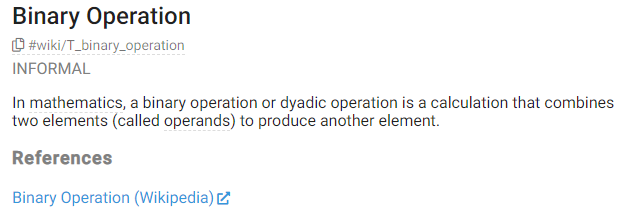
\includegraphics[height=5cm]{modal}}
\caption{Modal dialog box for the term binary operation. These boxes can also have content that uses all three types of links. }
\label{fig1}
\end{center}
\end{figure}

\subsubsection{Resource Expansion}

Instead of creating a link, this option expands the resource in place. For terms and propositions, the definition and the statement are added in place, respectively. For arguments, the premises, conclusion, and the argument text is added in place. Another option `ARG\_TEXT\_ONLY' can be used for to dislay only the argument text.



\paragraph{Example}
The following is a sample article where we uses re-use concepts and theorems already extracted from multiple sources (say, Wikipedia and the Oxford dictionary):

\begin{verbatim}
# Conic section

A conic section (or simply conic) is a curve obtained as the intersection of the
#(wiki/T_conical_surface, 'surface') of a #wiki/T_cone with a #wiki/T_plane. There are
three types of conic sections.


## Ellipse
#oxford/T_ellipse|EXPAND #wiki/P_ellipse_area|EXPAND


## Parabola
#oxford/T_parabola|EXPAND The area of a parabola is unbounded.

## Hyperbola  
#oxford/T_hyperbola|EXPAND The area of a hyperbola is unbounded.

\end{verbatim}

\paragraph{The above code is rendered as:}
\begin{mdframed}
\section*{Conic Section}
A conic section (or simply conic) is a curve obtained as the intersection of the \dashuline{surface} of a \dashuline{cone} with a \dashuline{plane}. There are three types of conic sections.

\subsection*{Ellipse}
An ellipse is a regular \dashuline{oval} shape, traced by a point moving in a plane so that the sum of its distances from two other points (the foci) is constant, or resulting when a cone is cut by an oblique plane which does not intersect the base.  The area $A_{ellipse}$ enclosed by an ellipse is $$A_{ellipse} = \pi a b$$where $a$ and $b$ are the lengths of the \dashuline{semi-major} and \dashuline{semi-minor} axes, respectively.

\subsection*{Parabola}
A parabola is a \dashuline{symmetrical} open plane curve formed by the intersection of a cone with a plane parallel to its side. The area of a parabola is unbounded.


\subsection*{Hyperbola}
A Hyperbola symmetrical open curve formed by the intersection of a circular cone with a plane at a smaller angle with its axis than the side of the cone. The area of a hyperbola is unbounded.

\end{mdframed}

\subsubsection{Status Indicators}

For propositions, a Truth Value Icon indicating whether or not there is a proof is added next to the link. Clicking on the icon brings up the proof as a graph of arguments. Similarly, an icon is added next to an argument which indicates whether the argument is valid or not. These options can be turned on or off depending on the user input and the context. Further details require details of the Sophize knowledge organization scheme which is not our focus here.


\subsection{Formal Language Support}

In formal languages, definitions of terms, statements of propositions, and supporting argument text may be parseable by an external parser. We can convert the externally parsed output into Markdown in such a case, where each term is automatically linked to the appropriate resource. This provides a delightful interface, where the user types in the native language, and the final output automatically allows users to explore all concepts than make up the input statement in depth. Currently, this is demonstrated in the use of Sophize Markdown with the Metamath language.

\subsection{\LaTeX\space Support}

While multiple applications extend Markdown to support TeX, there is no standardized syntax specification. However, Pandoc is the most widely used tool for converting \LaTeX\space to Markdown, and its specification is well documented and tested. Thus, we use their specification for our extension\cite{pandoc}:


\blockquote{Anything between two \$ characters will be treated as TeX math. The opening \$ must have a non-space character immediately to its right, while the closing \$ must have a non-space character immediately to its left, and must not be followed immediately by a digit. Thus, \$20,000 and \$30,000 won’t parse as math. If for some reason you need to enclose text in literal \$ characters, backslash-escape them and they won’t be treated as math delimiters.


For display math, use \$\$ delimiters. (In this case, the delimiters may be separated from the formula by whitespace. However, there can be no blank lines between the opening and closing \$\$ delimiters.)}


The following example summarizes the specification:
\begin{quote}
\begin{verbatim} 
Einstein's most famous equation is $E=mc^2$ but it is his handwritten theory of 
happiness is that fetched $1.3 million recently. While it may not fetch many \$s, I 
like the field equations more $$G_{\mu \nu }+\Lambda g_{\mu \nu }=\kappa T_{\mu \nu }$$
\end{verbatim}
\end{quote}


The above Markdown code is rendered as:
\begin{mdframed}
Einstein's most famous equation is $E=mc^2$ but it is his handwritten theory of happiness is
what fetched \$1.3 million recently. While it may not fetch many \$s, I like the field
equations more $$G_{\mu \nu }+\Lambda g_{\mu \nu }=\kappa T_{\mu \nu }$$
\end{mdframed}



\section{Sophize Collaboration Interface}

Sophize's communication interface is designed to allow multiple researchers to collaboratively solve a problem. In such open online collaborations, a lot of different ideas and approaches get introduced rapidly. Going through all these comments and making sense of the rapidly evolving ideas becomes a daunting task that can dissuade even the experts and the highly motivated. We believe that we have created a novel interface that can significantly mitigate this problem. The work is primarily influenced by recommendations made by Timothy Gowers and Terence Tao after organizing several Polymath projects\cite{polymath_blog}. We believe that the interface can aid many collaboration types - with few or many participants. We demonstrate the various features of this interface by incorporating actual data from a Polymath project at: \url{https://youtu.be/d3gaalJ7UQM}.


\subsubsection*{Requirements}

Helping users make sense of the conversation and allowing them to get up to speed with existing progress as quickly as possible is perhaps the most important requirement for managing online collaborations. To solve this problem, we need to organize the ideas in an intuitive way and to summarize the progress. A reader should be able to quickly grasp the current state, and project moderators need a way to manage the direction of various threads to avoid the big picture from being obscured.


Other technical requirements were discussed by some project participants and summarized by Tao on his blog\cite{whats_new_2009} (lightly edited):

\begin{itemize}

  \item \LaTeX\space support

  \item Group moderation

  \item Comment editing and preview

  \item Comment numbering and/or threading

  \item Wiki-like features, i.e., group-editable, publicly-viewable documents with version control

  \item Some way to view all recent comments or developments in a project

  \item Easy registration process

  \item Easy commenting process (i.e., no technical knowledge required)

  \item Permanent URLs for posts and comments (for link-back purposes)

\end{itemize}


We note that Sophize provides all the above features except that it doesn't yet allow users to look at the previous versions of documents. We summarize innovative features of the platform below:


\subsection{Hierarchical Page Organization}

As noted by Gowers, to make sense of the numerous ideas discussed, they need to be organized in a natural hierarchical way. The `proof discovery tree', as Gowers calls it \cite{gowers_weblog_2009}, would have a precise approach to the main problem, and each of the subproblems that come up would have its own trees. The leaves of the tree would thus be sub-problems that get solved without division into sub-problems.


Sophize brings the `Proof-discovery tree' to life by organizing the project using neatly organized wiki-like pages. Pages have a parent-child relationship allowing them to be organized like a tree. Discussion comments can be posted on any page, and moderators can rearrange them the way they think is best for the project. Moderators are also encouraged to add an overview on each page that quickly informs readers of the significant ideas that they should be familiar with before they start contributing.


\subsection{Comment Summaries}

Even after the hierarchical division of comments, some pages can still have a large number of comments, which make them difficult to follow. To overcome this problem, we allow project moderators to create summaries of discussions that have taken place so far. Comment summaries get embedded in the comment tree as a parent for comments they summarise. For example, they can club together multiple comment chains that are dead ends so that each reader doesn't waste time on them. Or they could summarize a sub-proof that was arrived at after dozens of comments.


\subsection{Sophize Markdown benefits}

Project collaborators get all the benefits of Sophize Markdown, such as easy linking of existing math content, \LaTeX\space support, and live preview of pages and comments being written or edited.


Comments in Sophize are numbered serially (starting with 1 for each collaboration), each comment can be referenced with the hashtag notation (e.g., `\#3' for the 3rd comment). Comments in an external project can be referenced by providing the project's URI (\#URI/COMMENT\_NUMBER).

Also, we make it extremely easy to extract terms, propositions and proofs from comments. These resources not only help in better understanding of the project, it also helps build Sophize's library.


\subsection{Reducing noise}

Sophize gives project moderators the usual tools like spam removal and fine-grained access control to manage participants. We also add a new feature where certain comments can be marked hidden. Often, threads of dozens of comments can be just noise because they were based on confused concepts or mistaken assumptions. Such comments should not be marked as spam. By marking such threads as `hidden', moderators can ensure that these are not shown by default. But any user can view them if they wish to.

\subsubsection*{Sources}
The Sophize Markdown parser and its Angular renderer source code are available under an MIT license at \url{https://github.com/Sophize/sophize-md-parser} and \url{https://github.com/Sophize/ngx-sophize-md-renderer}, respectively. The NPM packages for these projects are named `sophize-md-parser' and `ngx-sophize-md-renderer'.

\subsubsection*{Acknowledgements}
This publication resulted (in part) from research supported by the International Mathematical Union. We would like to thank Patrick Ion for encouraging us to publish our work and also for their help in organizing the content of the paper.

\bibliographystyle{alpha} 

\bibliography{mybib}

%inline the .bbl file directly for mailing to authors.

%\begin{thebibliography}{Com79}

%\bibitem[Com79]{Comer-btree}
%D.~Comer.
%\newblock The ubiquitous b-tree.
%\newblock {\em Computing Surveys}, 11(2):121--137, June 1979.


%\bibitem[Com79]{Comer-btree}
%D.~Comer. \newblock The ubiquitous b-tree. \newblock {\em Computing Surveys}, 11(2):121--137, June 1979.

%\bibitem[Knu73]{Knuth-vol3}
%D.~E. Knuth. \newblock {\em The Art of Computer Programming -- Volume 3 / Sorting and Searching}. \newblock Addison-Wesley, 1973.
%\end{thebibliography}

\end{document}
